\documentclass{article}\usepackage[]{graphicx}\usepackage[]{color}
%% maxwidth is the original width if it is less than linewidth
%% otherwise use linewidth (to make sure the graphics do not exceed the margin)
\makeatletter
\def\maxwidth{ %
  \ifdim\Gin@nat@width>\linewidth
    \linewidth
  \else
    \Gin@nat@width
  \fi
}
\makeatother

\definecolor{fgcolor}{rgb}{0.345, 0.345, 0.345}
\newcommand{\hlnum}[1]{\textcolor[rgb]{0.686,0.059,0.569}{#1}}%
\newcommand{\hlstr}[1]{\textcolor[rgb]{0.192,0.494,0.8}{#1}}%
\newcommand{\hlcom}[1]{\textcolor[rgb]{0.678,0.584,0.686}{\textit{#1}}}%
\newcommand{\hlopt}[1]{\textcolor[rgb]{0,0,0}{#1}}%
\newcommand{\hlstd}[1]{\textcolor[rgb]{0.345,0.345,0.345}{#1}}%
\newcommand{\hlkwa}[1]{\textcolor[rgb]{0.161,0.373,0.58}{\textbf{#1}}}%
\newcommand{\hlkwb}[1]{\textcolor[rgb]{0.69,0.353,0.396}{#1}}%
\newcommand{\hlkwc}[1]{\textcolor[rgb]{0.333,0.667,0.333}{#1}}%
\newcommand{\hlkwd}[1]{\textcolor[rgb]{0.737,0.353,0.396}{\textbf{#1}}}%

\usepackage{framed}
\makeatletter
\newenvironment{kframe}{%
 \def\at@end@of@kframe{}%
 \ifinner\ifhmode%
  \def\at@end@of@kframe{\end{minipage}}%
  \begin{minipage}{\columnwidth}%
 \fi\fi%
 \def\FrameCommand##1{\hskip\@totalleftmargin \hskip-\fboxsep
 \colorbox{shadecolor}{##1}\hskip-\fboxsep
     % There is no \\@totalrightmargin, so:
     \hskip-\linewidth \hskip-\@totalleftmargin \hskip\columnwidth}%
 \MakeFramed {\advance\hsize-\width
   \@totalleftmargin\z@ \linewidth\hsize
   \@setminipage}}%
 {\par\unskip\endMakeFramed%
 \at@end@of@kframe}
\makeatother

\definecolor{shadecolor}{rgb}{.97, .97, .97}
\definecolor{messagecolor}{rgb}{0, 0, 0}
\definecolor{warningcolor}{rgb}{1, 0, 1}
\definecolor{errorcolor}{rgb}{1, 0, 0}
\newenvironment{knitrout}{}{} % an empty environment to be redefined in TeX

\usepackage{alltt}
\usepackage{enumerate}
\usepackage{amsmath}
\IfFileExists{upquote.sty}{\usepackage{upquote}}{}
\begin{document}

\title{\huge \textbf{Stat 207 HW7} \\}
\author{\large Cheng Luo 912466499 \\ \large Fan Wu 912538518}
\maketitle

\newpage
\mbox{}
\newpage


\section{14.11}

\begin{enumerate}[(a)]

\item

\begin{knitrout}
\definecolor{shadecolor}{rgb}{0.969, 0.969, 0.969}\color{fgcolor}\begin{kframe}
\begin{alltt}
  \hlstd{dat} \hlkwb{=} \hlkwd{read.table}\hlstd{(}\hlstr{"CH14PR11.txt"}\hlstd{)}
  \hlkwd{names}\hlstd{(dat)} \hlkwb{=} \hlkwd{c}\hlstd{(}\hlstr{"X"}\hlstd{,} \hlstr{"n"}\hlstd{,} \hlstr{"Y"}\hlstd{)}
  \hlkwd{plot}\hlstd{(dat}\hlopt{$}\hlstd{X, dat}\hlopt{$}\hlstd{Y}\hlopt{/}\hlstd{dat}\hlopt{$}\hlstd{n)}
\end{alltt}
\end{kframe}
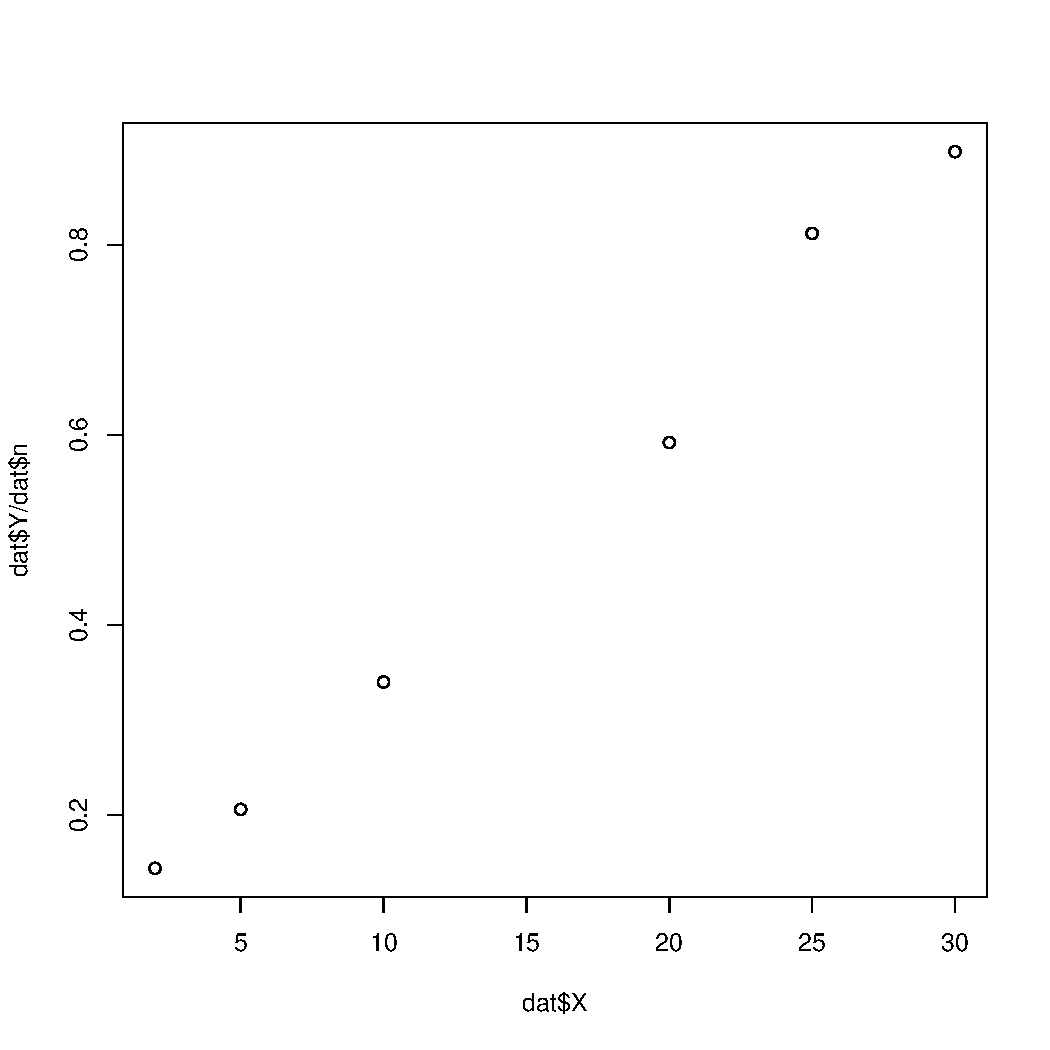
\includegraphics[width=\maxwidth]{figure/unnamed-chunk-1-1} 

\end{knitrout}

\qquad The plot support the analyst's belief that the logistic response functiion is appropriate.

\item

\begin{knitrout}
\definecolor{shadecolor}{rgb}{0.969, 0.969, 0.969}\color{fgcolor}\begin{kframe}
\begin{alltt}
  \hlstd{logit} \hlkwb{=} \hlkwd{glm}\hlstd{(Y}\hlopt{/}\hlstd{n} \hlopt{~} \hlstd{X,} \hlkwc{data} \hlstd{= dat,} \hlkwc{weight} \hlstd{= n ,} \hlkwc{family} \hlstd{=} \hlstr{"binomial"}\hlstd{)}
  \hlkwd{summary}\hlstd{(logit)}
\end{alltt}
\begin{verbatim}
## 
## Call:
## glm(formula = Y/n ~ X, family = "binomial", data = dat, weights = n)
## 
## Deviance Residuals: 
##       1        2        3        4        5        6  
##  0.1754   0.4330   0.5784  -2.9193   1.2710   1.2209  
## 
## Coefficients:
##              Estimate Std. Error z value Pr(>|z|)    
## (Intercept) -2.076565   0.084839  -24.48   <2e-16 ***
## X            0.135851   0.004772   28.47   <2e-16 ***
## ---
## Signif. codes:  0 '***' 0.001 '**' 0.01 '*' 0.05 '.' 0.1 ' ' 1
## 
## (Dispersion parameter for binomial family taken to be 1)
## 
##     Null deviance: 1108.171  on 5  degrees of freedom
## Residual deviance:   12.181  on 4  degrees of freedom
## AIC: 53.419
## 
## Number of Fisher Scoring iterations: 3
\end{verbatim}
\end{kframe}
\end{knitrout}

\qquad From the summary, the maximum likelihood estimates of $\hat{\beta}_0 = -2.0766$, $\hat{\beta}_1 = 0.1359$, $$\hat{\pi} = \frac{exp(\beta_0+\beta_1 X)}{1+exp(\beta_0+\beta_1 X)}=\frac{exp(-2.0766+0.1359 X)}{1+exp(-2.0766+0.1359 X)}$$

\item

\begin{knitrout}
\definecolor{shadecolor}{rgb}{0.969, 0.969, 0.969}\color{fgcolor}\begin{kframe}
\begin{alltt}
  \hlkwd{plot}\hlstd{(dat}\hlopt{$}\hlstd{X,} \hlkwd{fitted}\hlstd{(logit),} \hlkwc{ylim} \hlstd{=} \hlkwd{c}\hlstd{(}\hlnum{0}\hlstd{,} \hlnum{1}\hlstd{))}
  \hlkwd{points}\hlstd{(dat}\hlopt{$}\hlstd{X, dat}\hlopt{$}\hlstd{Y}\hlopt{/}\hlstd{dat}\hlopt{$}\hlstd{n,} \hlkwc{lwd} \hlstd{=} \hlnum{1}\hlstd{)}
\end{alltt}
\end{kframe}
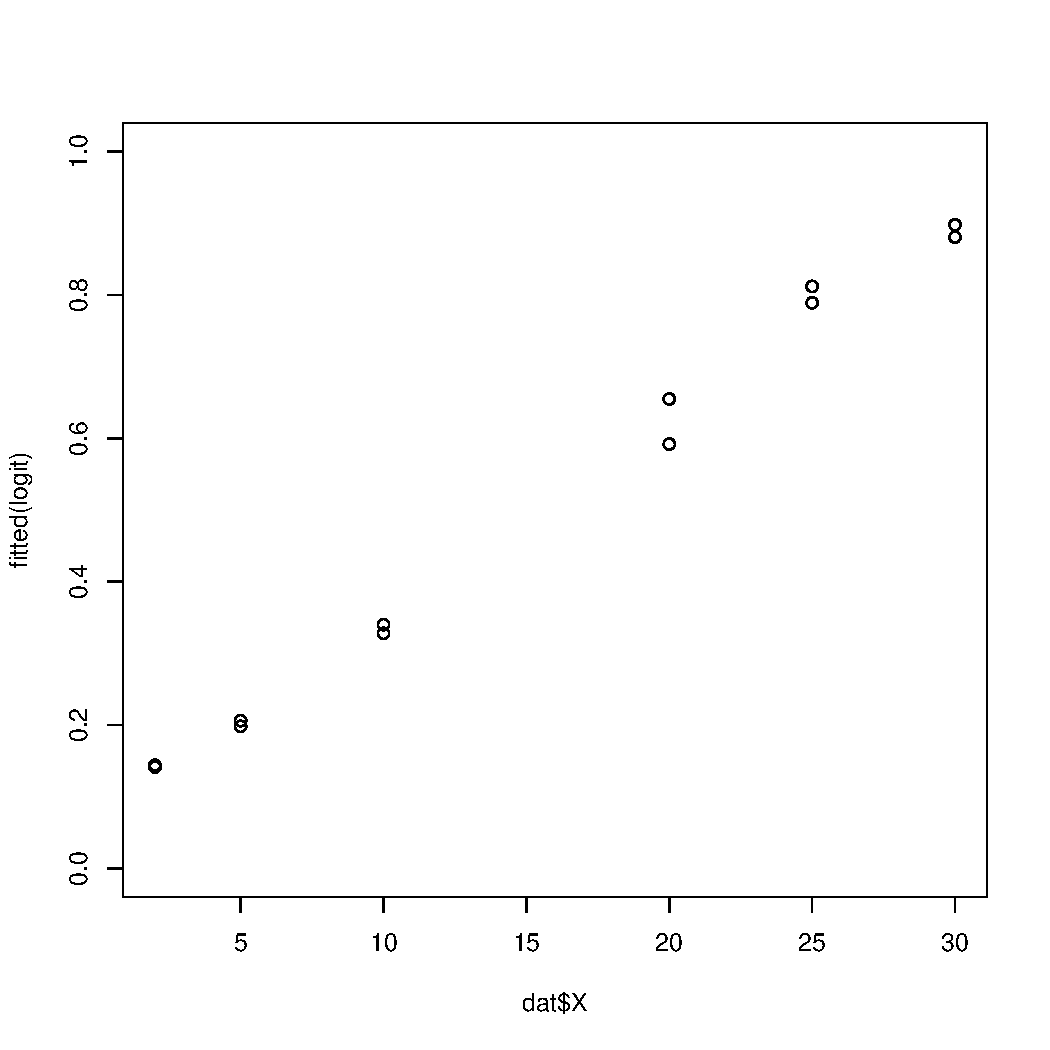
\includegraphics[width=\maxwidth]{figure/unnamed-chunk-3-1} 

\end{knitrout}

\qquad The fitted logistic response function appears to be well.

\item

\begin{knitrout}
\definecolor{shadecolor}{rgb}{0.969, 0.969, 0.969}\color{fgcolor}\begin{kframe}
\begin{alltt}
  \hlkwd{exp}\hlstd{(}\hlnum{0.1359}\hlstd{)}
\end{alltt}
\begin{verbatim}
## [1] 1.145567
\end{verbatim}
\end{kframe}
\end{knitrout}

\qquad $exp(\beta_1)=1.145567$, so that the odds of the bottles being returned is increased by 14.5567\% with each one deposit level increased.

\item

\begin{knitrout}
\definecolor{shadecolor}{rgb}{0.969, 0.969, 0.969}\color{fgcolor}\begin{kframe}
\begin{alltt}
  \hlstd{newdat} \hlkwb{=} \hlkwd{data.frame}\hlstd{(}\hlkwc{X} \hlstd{=} \hlnum{15}\hlstd{)}
  \hlkwd{predict}\hlstd{(logit,} \hlkwc{newdata} \hlstd{= newdat,} \hlkwc{type} \hlstd{=} \hlstr{"response"}\hlstd{)}
\end{alltt}
\begin{verbatim}
##         1 
## 0.4903005
\end{verbatim}
\end{kframe}
\end{knitrout}

\qquad The estimated probability that a bottle will be returned when the deposit is 15 cents is 0.4903005.

\item

\begin{knitrout}
\definecolor{shadecolor}{rgb}{0.969, 0.969, 0.969}\color{fgcolor}\begin{kframe}
\begin{alltt}
  \hlstd{newpi} \hlkwb{=} \hlnum{0.75}
  \hlstd{pi_2} \hlkwb{=} \hlkwd{log}\hlstd{(newpi}\hlopt{/}\hlstd{(}\hlnum{1}\hlopt{-}\hlstd{newpi))}
  \hlstd{(pi_2} \hlopt{-} \hlstd{(}\hlopt{-}\hlnum{2.0766}\hlstd{))}\hlopt{/}\hlnum{0.1359}
\end{alltt}
\begin{verbatim}
## [1] 23.36433
\end{verbatim}
\end{kframe}
\end{knitrout}

\qquad Estimate the amount of deposit for which 75\% of the bottles are expected to be returned is 23.36433.

\end{enumerate}

\section{14.14}

\begin{enumerate}[(a)]

\item

\begin{knitrout}
\definecolor{shadecolor}{rgb}{0.969, 0.969, 0.969}\color{fgcolor}\begin{kframe}
\begin{alltt}
  \hlstd{dat} \hlkwb{=} \hlkwd{read.table}\hlstd{(}\hlstr{"CH14PR14.txt"}\hlstd{)}
  \hlkwd{names}\hlstd{(dat)} \hlkwb{=} \hlkwd{c}\hlstd{(}\hlstr{"Y"}\hlstd{,} \hlstr{"X1"}\hlstd{,} \hlstr{"X2"}\hlstd{,} \hlstr{"X3"}\hlstd{)}
  \hlstd{logit} \hlkwb{=} \hlkwd{glm}\hlstd{(Y} \hlopt{~} \hlstd{X1} \hlopt{+} \hlstd{X2} \hlopt{+} \hlstd{X3,} \hlkwc{data} \hlstd{= dat,} \hlkwc{family} \hlstd{=} \hlstr{"binomial"}\hlstd{)}
  \hlkwd{summary}\hlstd{(logit)}
\end{alltt}
\begin{verbatim}
## 
## Call:
## glm(formula = Y ~ X1 + X2 + X3, family = "binomial", data = dat)
## 
## Deviance Residuals: 
##     Min       1Q   Median       3Q      Max  
## -1.4037  -0.5637  -0.3352  -0.1542   2.9394  
## 
## Coefficients:
##             Estimate Std. Error z value Pr(>|z|)   
## (Intercept) -1.17716    2.98242  -0.395  0.69307   
## X1           0.07279    0.03038   2.396  0.01658 * 
## X2          -0.09899    0.03348  -2.957  0.00311 **
## X3           0.43397    0.52179   0.832  0.40558   
## ---
## Signif. codes:  0 '***' 0.001 '**' 0.01 '*' 0.05 '.' 0.1 ' ' 1
## 
## (Dispersion parameter for binomial family taken to be 1)
## 
##     Null deviance: 134.94  on 158  degrees of freedom
## Residual deviance: 105.09  on 155  degrees of freedom
## AIC: 113.09
## 
## Number of Fisher Scoring iterations: 6
\end{verbatim}
\end{kframe}
\end{knitrout}

\qquad From the summary, the maximum likelihood estimates $\hat{\beta}_0 = -1.17716 $, $\hat{\beta}_1 = 0.07279$, $\hat{\beta}_2 = -0.09899 $, $\hat{\beta}_4 = 0.43397 $ $$\hat{\pi} = \frac{exp(\beta_0+\beta_1 X1 + \beta_2 X2 + \beta_3 X3)}{1+exp(\beta_0+\beta_1 X1 + \beta_2 X2 + \beta_3 X3)}=\frac{exp(-1.17716+0.07279 X1 - 0.09899 X2 +0.43397 X3)}{1+exp(-1.17716+0.07279 X1 - 0.09899 X2 +0.43397 X3)}$$

\item

\begin{knitrout}
\definecolor{shadecolor}{rgb}{0.969, 0.969, 0.969}\color{fgcolor}\begin{kframe}
\begin{alltt}
  \hlkwd{exp}\hlstd{(}\hlnum{0.07279}\hlstd{)}
\end{alltt}
\begin{verbatim}
## [1] 1.075505
\end{verbatim}
\begin{alltt}
  \hlkwd{exp}\hlstd{(}\hlopt{-}\hlnum{0.09899} \hlstd{)}
\end{alltt}
\begin{verbatim}
## [1] 0.9057518
\end{verbatim}
\begin{alltt}
  \hlkwd{exp}\hlstd{(}\hlnum{0.43397}\hlstd{)}
\end{alltt}
\begin{verbatim}
## [1] 1.543373
\end{verbatim}
\end{kframe}
\end{knitrout}

\begin{itemize}
\item
$exp(\beta_1)=1.075505$, so that the odds of getting a flu shot is increased by 7.5\% with each one age increased.
\item
$exp(\beta_2)=0.9057518$, so that the odds of getting a flu shot is decreased by 9.4\% with each one health awareness index increased.
\item
$exp(\beta_3)=1.543373$, so that the odds of getting a flu shot is increased by 54.3\% from woman to man.
\end{itemize}

\item

\begin{knitrout}
\definecolor{shadecolor}{rgb}{0.969, 0.969, 0.969}\color{fgcolor}\begin{kframe}
\begin{alltt}
  \hlstd{newdat} \hlkwb{=} \hlkwd{data.frame}\hlstd{(}\hlkwc{X1} \hlstd{=} \hlnum{55}\hlstd{,} \hlkwc{X2} \hlstd{=} \hlnum{60}\hlstd{,} \hlkwc{X3} \hlstd{=} \hlnum{1}\hlstd{)}
  \hlkwd{predict}\hlstd{(logit,} \hlkwc{newdata} \hlstd{= newdat,} \hlkwc{type} \hlstd{=} \hlstr{"response"}\hlstd{)}
\end{alltt}
\begin{verbatim}
##          1 
## 0.06422197
\end{verbatim}
\end{kframe}
\end{knitrout}

\qquad The estimated probability with X1=55, X2=60 and X3=1 is 0.06422197 .

\end{enumerate}

\section{14.17}

\begin{enumerate}[(a)]

\item

\begin{knitrout}
\definecolor{shadecolor}{rgb}{0.969, 0.969, 0.969}\color{fgcolor}\begin{kframe}
\begin{alltt}
  \hlstd{dat} \hlkwb{=} \hlkwd{read.table}\hlstd{(}\hlstr{"CH14PR11.txt"}\hlstd{)}
  \hlkwd{names}\hlstd{(dat)} \hlkwb{=} \hlkwd{c}\hlstd{(}\hlstr{"X"}\hlstd{,} \hlstr{"n"}\hlstd{,} \hlstr{"Y"}\hlstd{)}
  \hlstd{logit} \hlkwb{=} \hlkwd{glm}\hlstd{(Y}\hlopt{/}\hlstd{n} \hlopt{~} \hlstd{X,} \hlkwc{weight}\hlstd{=n,} \hlkwc{data} \hlstd{= dat,} \hlkwc{family} \hlstd{=} \hlstr{"binomial"}\hlstd{)}
  \hlkwd{summary}\hlstd{(logit)}
\end{alltt}
\begin{verbatim}
## 
## Call:
## glm(formula = Y/n ~ X, family = "binomial", data = dat, weights = n)
## 
## Deviance Residuals: 
##       1        2        3        4        5        6  
##  0.1754   0.4330   0.5784  -2.9193   1.2710   1.2209  
## 
## Coefficients:
##              Estimate Std. Error z value Pr(>|z|)    
## (Intercept) -2.076565   0.084839  -24.48   <2e-16 ***
## X            0.135851   0.004772   28.47   <2e-16 ***
## ---
## Signif. codes:  0 '***' 0.001 '**' 0.01 '*' 0.05 '.' 0.1 ' ' 1
## 
## (Dispersion parameter for binomial family taken to be 1)
## 
##     Null deviance: 1108.171  on 5  degrees of freedom
## Residual deviance:   12.181  on 4  degrees of freedom
## AIC: 53.419
## 
## Number of Fisher Scoring iterations: 3
\end{verbatim}
\begin{alltt}
  \hlstd{b1} \hlkwb{=} \hlnum{0.1359}
  \hlstd{s1} \hlkwb{=} \hlnum{0.004772}
  \hlstd{z} \hlkwb{=} \hlkwd{qnorm}\hlstd{(}\hlnum{1}\hlopt{-}\hlnum{0.05}\hlopt{/}\hlnum{2}\hlstd{)}
  \hlkwd{c}\hlstd{(b1}\hlopt{-}\hlstd{s1}\hlopt{*}\hlstd{z, b1}\hlopt{+}\hlstd{s1}\hlopt{*}\hlstd{z)}
\end{alltt}
\begin{verbatim}
## [1] 0.1265471 0.1452529
\end{verbatim}
\begin{alltt}
  \hlkwd{c}\hlstd{(}\hlkwd{exp}\hlstd{(b1}\hlopt{-}\hlstd{s1}\hlopt{*}\hlstd{z),} \hlkwd{exp}\hlstd{(b1}\hlopt{+}\hlstd{s1}\hlopt{*}\hlstd{z))}
\end{alltt}
\begin{verbatim}
## [1] 1.134903 1.156332
\end{verbatim}
\end{kframe}
\end{knitrout}

\qquad From summary(logit), we get $s(b_1) = 0.004772, b_1 = 0.1359$, based on $b_k \pm z(1-\alpha/2)s{b_k}$, we conclude that we are 95 \% confident that $\beta_1$ is between 0.1265471 and 0.1452529, and corresponding confidence limits for the odds ratio $exp(\beta_1)$ is between 1.134903 and 1.156332.

\item

\begin{knitrout}
\definecolor{shadecolor}{rgb}{0.969, 0.969, 0.969}\color{fgcolor}\begin{kframe}
\begin{alltt}
  \hlkwd{qnorm}\hlstd{(}\hlnum{1}\hlopt{-}\hlnum{0.05}\hlopt{/}\hlnum{2}\hlstd{)}
\end{alltt}
\begin{verbatim}
## [1] 1.959964
\end{verbatim}
\end{kframe}
\end{knitrout}

\begin{center}
$H_0$:$\beta_1=0$

VS. $H_1$:$\beta_1 \ne 0$

$z^*=\frac{b_1}{s(b_1)} = 0.1359/0.004772   = 28.47863$

we can reject $H_0$ if $|z^*| > Z(1-0.05/2)=1.959964$,otherwise reject$H_1$

so that reject $H_0$ because $|z^*|>1.959964$,

therefore, X1 can not be dropped from the regression model, and the P-value is 2e-16
\end{center}

\item

\begin{knitrout}
\definecolor{shadecolor}{rgb}{0.969, 0.969, 0.969}\color{fgcolor}\begin{kframe}
\begin{alltt}
  \hlkwd{logLik}\hlstd{(logit)}
\end{alltt}
\begin{verbatim}
## 'log Lik.' -24.70937 (df=2)
\end{verbatim}
\begin{alltt}
  \hlstd{logitR} \hlkwb{=} \hlkwd{glm}\hlstd{(Y}\hlopt{/}\hlstd{n} \hlopt{~} \hlnum{1}\hlstd{,} \hlkwc{weight} \hlstd{= n,} \hlkwc{data} \hlstd{= dat,} \hlkwc{family} \hlstd{=} \hlstr{"binomial"}\hlstd{)}
  \hlkwd{logLik}\hlstd{(logitR)}
\end{alltt}
\begin{verbatim}
## 'log Lik.' -572.7044 (df=1)
\end{verbatim}
\begin{alltt}
  \hlkwd{qchisq}\hlstd{(}\hlnum{1}\hlopt{-}\hlnum{0.05}\hlstd{,} \hlnum{2}\hlopt{-}\hlnum{1}\hlstd{)}
\end{alltt}
\begin{verbatim}
## [1] 3.841459
\end{verbatim}
\begin{alltt}
  \hlkwd{pchisq}\hlstd{(}\hlnum{1095.99}\hlstd{,} \hlnum{1}\hlstd{,} \hlkwc{lower.tail} \hlstd{=} \hlnum{FALSE}\hlstd{)}
\end{alltt}
\begin{verbatim}
## [1] 2.457179e-240
\end{verbatim}
\end{kframe}
\end{knitrout}

\begin{center}
$H_0$:$\beta_1=0$

VS. $H_1$:$\beta_1 \ne 0$

The full model: $\pi = [1 + exp(-(\beta_0 + \beta_1 X1))]^{-1} $

ln(L(F))= -24.70937

The reduced model: $\pi = [1 + exp(-(\beta_0))]^{-1} $

ln(L(R))= -572.7044

$G^2$ = -2(ln(L(R)-ln(L(F)))) = 1095.99

we can reject $H_0$ if $G^2 > \chi^2(1-0.05, 2-1)=3.8415$,otherwise reject$H_1$

so that reject $H_0$ because $G^2 >3.8415$,

therefore, X1 cannot be dropped from the regression model, and the P-value is 2.457179e-240.And the result is different from the result we get in (b).
\end{center}

\end{enumerate}

\section{14.20}

\begin{enumerate}[(a)]

\item

\begin{knitrout}
\definecolor{shadecolor}{rgb}{0.969, 0.969, 0.969}\color{fgcolor}\begin{kframe}
\begin{alltt}
  \hlstd{dat} \hlkwb{=} \hlkwd{read.table}\hlstd{(}\hlstr{"CH14PR14.txt"}\hlstd{)}
  \hlkwd{names}\hlstd{(dat)} \hlkwb{=} \hlkwd{c}\hlstd{(}\hlstr{"Y"}\hlstd{,} \hlstr{"X1"}\hlstd{,} \hlstr{"X2"}\hlstd{,} \hlstr{"X3"}\hlstd{)}
  \hlstd{logit} \hlkwb{=} \hlkwd{glm}\hlstd{(Y} \hlopt{~} \hlstd{X1} \hlopt{+} \hlstd{X2} \hlopt{+} \hlstd{X3,} \hlkwc{data} \hlstd{= dat,} \hlkwc{family} \hlstd{=} \hlstr{"binomial"}\hlstd{)}
  \hlkwd{summary}\hlstd{(logit)}
\end{alltt}
\begin{verbatim}
## 
## Call:
## glm(formula = Y ~ X1 + X2 + X3, family = "binomial", data = dat)
## 
## Deviance Residuals: 
##     Min       1Q   Median       3Q      Max  
## -1.4037  -0.5637  -0.3352  -0.1542   2.9394  
## 
## Coefficients:
##             Estimate Std. Error z value Pr(>|z|)   
## (Intercept) -1.17716    2.98242  -0.395  0.69307   
## X1           0.07279    0.03038   2.396  0.01658 * 
## X2          -0.09899    0.03348  -2.957  0.00311 **
## X3           0.43397    0.52179   0.832  0.40558   
## ---
## Signif. codes:  0 '***' 0.001 '**' 0.01 '*' 0.05 '.' 0.1 ' ' 1
## 
## (Dispersion parameter for binomial family taken to be 1)
## 
##     Null deviance: 134.94  on 158  degrees of freedom
## Residual deviance: 105.09  on 155  degrees of freedom
## AIC: 113.09
## 
## Number of Fisher Scoring iterations: 6
\end{verbatim}
\end{kframe}
\end{knitrout}

\qquad $z(1-\frac{0.1}{2*2})=0.975, s(b_1)=0.03038, s(b_2)=0.03348$
$$exp(30∗(0.0728−0.03038∗1.96))<exp(30\beta_1)<exp(30∗(0.0728+0.03038∗1.96))$$
$$1.4878<exp(30\beta_1)<52.9837$$
$$exp(25∗(−0.099−0.03348∗1.96))<exp(25\beta_2)<exp(25∗(0.0728+0.03348∗1.96))$$
$$0.0163 <exp(25\beta_2)< 31.824$$
\item

\begin{knitrout}
\definecolor{shadecolor}{rgb}{0.969, 0.969, 0.969}\color{fgcolor}\begin{kframe}
\begin{alltt}
  \hlkwd{qnorm}\hlstd{(}\hlnum{1}\hlopt{-}\hlnum{0.05}\hlopt{/}\hlnum{2}\hlstd{)}
\end{alltt}
\begin{verbatim}
## [1] 1.959964
\end{verbatim}
\end{kframe}
\end{knitrout}

\begin{center}
$H_0$:$\beta_3=0$

VS. $H_1$:$\beta_3 \ne 0$

$z^*=\frac{b_3}{s(b_3)} = 0.43397/0.52179   = 0.8316947$

we can reject $H_0$ if $|z^*| > Z(1-0.05/2)=1.959964$,otherwise reject$H_1$

so that reject $H_1$ because $|z^*|<1.959964$,

therefore, X3 can be dropped from the regression model, and the P-value is 0.40558  
\end{center}

\item

\begin{knitrout}
\definecolor{shadecolor}{rgb}{0.969, 0.969, 0.969}\color{fgcolor}\begin{kframe}
\begin{alltt}
  \hlkwd{logLik}\hlstd{(logit)}
\end{alltt}
\begin{verbatim}
## 'log Lik.' -52.54659 (df=4)
\end{verbatim}
\begin{alltt}
  \hlstd{logitR} \hlkwb{=} \hlkwd{glm}\hlstd{(Y} \hlopt{~} \hlstd{X1}\hlopt{+}\hlstd{X2,} \hlkwc{data} \hlstd{= dat,} \hlkwc{family} \hlstd{=} \hlstr{"binomial"}\hlstd{)}
  \hlkwd{logLik}\hlstd{(logitR)}
\end{alltt}
\begin{verbatim}
## 'log Lik.' -52.89769 (df=3)
\end{verbatim}
\begin{alltt}
  \hlkwd{qchisq}\hlstd{(}\hlnum{1}\hlopt{-}\hlnum{0.05}\hlstd{,} \hlnum{4}\hlopt{-}\hlnum{3}\hlstd{)}
\end{alltt}
\begin{verbatim}
## [1] 3.841459
\end{verbatim}
\begin{alltt}
  \hlkwd{pchisq}\hlstd{(}\hlnum{0.70236}\hlstd{,} \hlnum{1}\hlstd{,} \hlkwc{lower.tail} \hlstd{=} \hlnum{FALSE}\hlstd{)}
\end{alltt}
\begin{verbatim}
## [1] 0.4019918
\end{verbatim}
\end{kframe}
\end{knitrout}

\begin{center}
$H_0$:$\beta_3=0$

VS. $H_1$:$\beta_3 \ne 0$

The full model: $\pi = [1 + exp(-(\beta_0 + \beta_1 X1 + \beta_2 X2 + \beta_3 X3))]^{-1} $

ln(L(F))= -52.54659

The reduced model: $\pi = [1 + exp(-(\beta_0 + \beta_1 X1 + \beta_2 X2))]^{-1} $

ln(L(R))= -52.89769

$G^2$ = -2(ln(L(R)-ln(L(F)))) = 0.70236

we can reject $H_0$ if $G^2 > \chi^2(1-0.05, 4-3)=3.8415$,otherwise reject$H_1$

so that reject $H_1$ because $G^2 < 3.8415$,

therefore, X3 can be dropped from the regression model, and the P-value is 0.4019918.And the result is the same as the result we get in (b).
\end{center}

\item

\begin{knitrout}
\definecolor{shadecolor}{rgb}{0.969, 0.969, 0.969}\color{fgcolor}\begin{kframe}
\begin{alltt}
  \hlstd{logitF} \hlkwb{=} \hlkwd{glm}\hlstd{(Y} \hlopt{~} \hlstd{X1}\hlopt{+}\hlstd{X2}\hlopt{+}\hlkwd{I}\hlstd{(X1}\hlopt{^}\hlnum{2}\hlstd{)}\hlopt{+}\hlkwd{I}\hlstd{(X2}\hlopt{^}\hlnum{2}\hlstd{)}\hlopt{+}\hlkwd{I}\hlstd{(X1}\hlopt{*}\hlstd{X2),} \hlkwc{data} \hlstd{= dat,} \hlkwc{family} \hlstd{=} \hlstr{"binomial"}\hlstd{)}
  \hlkwd{logLik}\hlstd{(logitF)}
\end{alltt}
\begin{verbatim}
## 'log Lik.' -52.13072 (df=6)
\end{verbatim}
\begin{alltt}
  \hlstd{logitR} \hlkwb{=} \hlkwd{glm}\hlstd{(Y} \hlopt{~} \hlstd{X1}\hlopt{+}\hlstd{X2,} \hlkwc{data} \hlstd{= dat,} \hlkwc{family} \hlstd{=} \hlstr{"binomial"}\hlstd{)}
  \hlkwd{logLik}\hlstd{(logitR)}
\end{alltt}
\begin{verbatim}
## 'log Lik.' -52.89769 (df=3)
\end{verbatim}
\begin{alltt}
  \hlkwd{qchisq}\hlstd{(}\hlnum{1}\hlopt{-}\hlnum{0.05}\hlstd{,} \hlnum{6}\hlopt{-}\hlnum{3}\hlstd{)}
\end{alltt}
\begin{verbatim}
## [1] 7.814728
\end{verbatim}
\begin{alltt}
  \hlkwd{pchisq}\hlstd{(}\hlnum{1.53394}\hlstd{,} \hlnum{3}\hlstd{,} \hlkwc{lower.tail} \hlstd{=} \hlnum{FALSE}\hlstd{)}
\end{alltt}
\begin{verbatim}
## [1] 0.6744594
\end{verbatim}
\end{kframe}
\end{knitrout}

\begin{center}
$H_0$:$\beta_3=\beta_4=\beta_5=0$

VS. $H_1$:$not all \beta_3,\beta_4,\beta_5 equal 0$

The full model: $\pi = [1 + exp(-(\beta_0 + \beta_1 X1 + \beta_2 X2 + \beta_3 X1^2 + \beta_4 X2^2 + \beta_5 X1*X2))]^{-1} $

ln(L(F))= -52.13072

The reduced model: $\pi = [1 + exp(-(\beta_0 + \beta_1 X1 + \beta_2 X2))]^{-1} $

ln(L(R))= -52.89769

$G^2$ = -2(ln(L(R)-ln(L(F)))) = 1.53394

we can reject $H_0$ if $G^2 > \chi^2(1-0.05, 6-3)=7.814728$,otherwise reject$H_1$

so that reject $H_1$ because $G^2 < 7.814728$,

therefore, $X1^2,X2^2,I(X1*X2)$ can be dropped from the regression model, and the P-value is 0.6744594.And the result is the same as the result we get in (b).
\end{center}

\end{enumerate}

\section{14.22}

\begin{enumerate}[(a)]

\item

\begin{knitrout}
\definecolor{shadecolor}{rgb}{0.969, 0.969, 0.969}\color{fgcolor}\begin{kframe}
\begin{alltt}
  \hlstd{dat} \hlkwb{=} \hlkwd{read.table}\hlstd{(}\hlstr{"CH14PR14.txt"}\hlstd{)}
  \hlkwd{names}\hlstd{(dat)} \hlkwb{=} \hlkwd{c}\hlstd{(}\hlstr{"y"}\hlstd{,} \hlstr{"x1"}\hlstd{,} \hlstr{"x2"}\hlstd{,} \hlstr{"x3"}\hlstd{)}
  \hlstd{dat.new} \hlkwb{=} \hlkwd{scale}\hlstd{(dat[,} \hlnum{2}\hlopt{:}\hlnum{4}\hlstd{],} \hlkwc{scale} \hlstd{=} \hlnum{FALSE}\hlstd{)}
  \hlstd{dat.new} \hlkwb{=} \hlkwd{as.data.frame}\hlstd{(}\hlkwd{cbind}\hlstd{(dat}\hlopt{$}\hlstd{y, dat.new))}
  \hlkwd{names}\hlstd{(dat.new)} \hlkwb{=} \hlkwd{c}\hlstd{(}\hlstr{"y"}\hlstd{,} \hlstr{"x1"}\hlstd{,} \hlstr{"x2"}\hlstd{,} \hlstr{"x3"}\hlstd{)}

  \hlstd{alpha} \hlkwb{=} \hlnum{.1}
  \hlstd{wrap.foo} \hlkwb{=} \hlkwa{function}\hlstd{(}\hlkwc{formula}\hlstd{,} \hlkwc{dat.new.} \hlstd{= dat.new)}
  \hlstd{\{}
    \hlstd{model} \hlkwb{=} \hlkwd{glm}\hlstd{(formula,} \hlkwc{family} \hlstd{= binomial,} \hlkwc{data} \hlstd{= dat.new.)}
    \hlstd{p.val} \hlkwb{=} \hlkwd{summary}\hlstd{(model)}\hlopt{$}\hlstd{coef}
    \hlstd{p.val[}\hlkwd{nrow}\hlstd{(p.val),} \hlnum{4}\hlstd{]}
  \hlstd{\}}
  \hlstd{tmp} \hlkwb{=} \hlkwd{c}\hlstd{(}\hlkwd{wrap.foo}\hlstd{(y} \hlopt{~} \hlstd{x1),}
          \hlkwd{wrap.foo}\hlstd{(y} \hlopt{~} \hlstd{x2),}
          \hlkwd{wrap.foo}\hlstd{(y} \hlopt{~} \hlkwd{I}\hlstd{(x1}\hlopt{*}\hlstd{x2)),}
          \hlkwd{wrap.foo}\hlstd{(y} \hlopt{~} \hlkwd{I}\hlstd{(x1}\hlopt{^}\hlnum{2}\hlstd{)),}
          \hlkwd{wrap.foo}\hlstd{(y} \hlopt{~} \hlkwd{I}\hlstd{(x2}\hlopt{^}\hlnum{2}\hlstd{)),}
          \hlkwd{wrap.foo}\hlstd{(y} \hlopt{~} \hlkwd{I}\hlstd{(x1}\hlopt{^}\hlnum{2}\hlstd{)}\hlopt{:}\hlkwd{I}\hlstd{(x2}\hlopt{^}\hlnum{2}\hlstd{)))}
  \hlkwd{any}\hlstd{(tmp} \hlopt{<} \hlstd{alpha)}
\end{alltt}
\begin{verbatim}
## [1] TRUE
\end{verbatim}
\begin{alltt}
  \hlkwd{which.min}\hlstd{(tmp)}
\end{alltt}
\begin{verbatim}
## [1] 1
\end{verbatim}
\begin{alltt}
  \hlstd{tmp} \hlkwb{=} \hlkwd{c}\hlstd{(}\hlkwd{wrap.foo}\hlstd{(y} \hlopt{~} \hlstd{x1} \hlopt{+} \hlstd{x2),}
          \hlkwd{wrap.foo}\hlstd{(y} \hlopt{~} \hlstd{x1} \hlopt{+} \hlkwd{I}\hlstd{(x1}\hlopt{*}\hlstd{x2)),}
          \hlkwd{wrap.foo}\hlstd{(y} \hlopt{~} \hlstd{x1} \hlopt{+} \hlkwd{I}\hlstd{(x1}\hlopt{^}\hlnum{2}\hlstd{)),}
          \hlkwd{wrap.foo}\hlstd{(y} \hlopt{~} \hlstd{x1} \hlopt{+} \hlkwd{I}\hlstd{(x2}\hlopt{^}\hlnum{2}\hlstd{))}
          \hlstd{)}
  \hlkwd{any}\hlstd{(tmp} \hlopt{<} \hlstd{alpha)}
\end{alltt}
\begin{verbatim}
## [1] TRUE
\end{verbatim}
\begin{alltt}
  \hlkwd{which.min}\hlstd{(tmp)}
\end{alltt}
\begin{verbatim}
## [1] 1
\end{verbatim}
\begin{alltt}
  \hlstd{tmp} \hlkwb{=} \hlkwd{c}\hlstd{(}\hlkwd{wrap.foo}\hlstd{(y} \hlopt{~} \hlstd{x1} \hlopt{+} \hlstd{x2} \hlopt{+} \hlkwd{I}\hlstd{(x1}\hlopt{*}\hlstd{x2)),}
          \hlkwd{wrap.foo}\hlstd{(y} \hlopt{~} \hlstd{x1} \hlopt{+} \hlstd{x2} \hlopt{+} \hlkwd{I}\hlstd{(x1}\hlopt{^}\hlnum{2}\hlstd{)),}
          \hlkwd{wrap.foo}\hlstd{(y} \hlopt{~} \hlstd{x1} \hlopt{+} \hlstd{x2} \hlopt{+} \hlkwd{I}\hlstd{(x2}\hlopt{^}\hlnum{2}\hlstd{))}
          \hlstd{)}
  \hlkwd{any}\hlstd{(tmp} \hlopt{<} \hlstd{alpha)}
\end{alltt}
\begin{verbatim}
## [1] FALSE
\end{verbatim}
\end{kframe}
\end{knitrout}

\qquad X1 enters in step 1 ; X2 enters in step 2; no variables satisfy criterion for entry in step 3.

\item

\begin{knitrout}
\definecolor{shadecolor}{rgb}{0.969, 0.969, 0.969}\color{fgcolor}\begin{kframe}
\begin{alltt}
  \hlstd{wrap.foo} \hlkwb{=} \hlkwa{function}\hlstd{(}\hlkwc{formula}\hlstd{,} \hlkwc{dat.new.} \hlstd{= dat.new)}
  \hlstd{\{}
    \hlstd{model} \hlkwb{=} \hlkwd{glm}\hlstd{(formula,} \hlkwc{family} \hlstd{= binomial,} \hlkwc{data} \hlstd{= dat.new.)}
    \hlstd{p.val} \hlkwb{=} \hlkwd{summary}\hlstd{(model)}\hlopt{$}\hlstd{coef}
    \hlstd{p.val} \hlkwb{=} \hlstd{p.val[,} \hlnum{4}\hlstd{]}
    \hlstd{p.val[}\hlopt{-}\hlnum{1}\hlstd{]}
  \hlstd{\}}

  \hlstd{tmp} \hlkwb{=} \hlkwd{wrap.foo}\hlstd{(y} \hlopt{~} \hlstd{x1} \hlopt{+} \hlstd{x2} \hlopt{+} \hlkwd{I}\hlstd{(x1}\hlopt{*}\hlstd{x2)} \hlopt{+} \hlkwd{I}\hlstd{(x1}\hlopt{^}\hlnum{2}\hlstd{)} \hlopt{+} \hlkwd{I}\hlstd{(x2}\hlopt{^}\hlnum{2}\hlstd{))}
  \hlkwd{any}\hlstd{(tmp} \hlopt{>} \hlstd{alpha)}
\end{alltt}
\begin{verbatim}
## [1] TRUE
\end{verbatim}
\begin{alltt}
  \hlkwd{which.max}\hlstd{(tmp)}
\end{alltt}
\begin{verbatim}
## I(x1^2) 
##       4
\end{verbatim}
\begin{alltt}
  \hlstd{tmp} \hlkwb{=} \hlkwd{wrap.foo}\hlstd{(y} \hlopt{~} \hlstd{x1} \hlopt{+} \hlstd{x2} \hlopt{+} \hlkwd{I}\hlstd{(x1}\hlopt{*}\hlstd{x2)} \hlopt{+} \hlkwd{I}\hlstd{(x2}\hlopt{^}\hlnum{2}\hlstd{))}
  \hlkwd{any}\hlstd{(tmp} \hlopt{>} \hlstd{alpha)}
\end{alltt}
\begin{verbatim}
## [1] TRUE
\end{verbatim}
\begin{alltt}
  \hlkwd{which.max}\hlstd{(tmp)}
\end{alltt}
\begin{verbatim}
## I(x1 * x2) 
##          3
\end{verbatim}
\begin{alltt}
  \hlstd{tmp} \hlkwb{=} \hlkwd{wrap.foo}\hlstd{(y} \hlopt{~} \hlstd{x1} \hlopt{+} \hlstd{x2} \hlopt{+} \hlkwd{I}\hlstd{(x2}\hlopt{^}\hlnum{2}\hlstd{))}
  \hlkwd{any}\hlstd{(tmp} \hlopt{>} \hlstd{alpha)}
\end{alltt}
\begin{verbatim}
## [1] TRUE
\end{verbatim}
\begin{alltt}
  \hlkwd{which.max}\hlstd{(tmp)}
\end{alltt}
\begin{verbatim}
## I(x2^2) 
##       3
\end{verbatim}
\begin{alltt}
  \hlstd{tmp} \hlkwb{=} \hlkwd{wrap.foo}\hlstd{(y} \hlopt{~} \hlstd{x1} \hlopt{+} \hlstd{x2)}
  \hlkwd{any}\hlstd{(tmp} \hlopt{>} \hlstd{alpha)}
\end{alltt}
\begin{verbatim}
## [1] FALSE
\end{verbatim}
\end{kframe}
\end{knitrout}

\qquad X11 is deleted in step 1; X12 is deleted in step 2; X3 is deleted in step 3; X22 is deleted in step 4; X1 and X2 are retained in the model.

\item

\begin{knitrout}
\definecolor{shadecolor}{rgb}{0.969, 0.969, 0.969}\color{fgcolor}\begin{kframe}
\begin{alltt}
  \hlstd{model} \hlkwb{=} \hlkwd{glm}\hlstd{(y} \hlopt{~} \hlstd{x1} \hlopt{+} \hlstd{x2} \hlopt{+} \hlkwd{I}\hlstd{(x1}\hlopt{*}\hlstd{x2)} \hlopt{+} \hlkwd{I}\hlstd{(x1}\hlopt{^}\hlnum{2}\hlstd{)} \hlopt{+} \hlkwd{I}\hlstd{(x2}\hlopt{^}\hlnum{2}\hlstd{)} \hlopt{+} \hlkwd{I}\hlstd{(x1}\hlopt{^}\hlnum{2}\hlopt{*}\hlstd{x2}\hlopt{^}\hlnum{2}\hlstd{),}
              \hlkwc{family} \hlstd{= binomial,} \hlkwc{data} \hlstd{= dat.new)}
  \hlkwd{step}\hlstd{(model)}
\end{alltt}
\begin{verbatim}
## Start:  AIC=116.67
## y ~ x1 + x2 + I(x1 * x2) + I(x1^2) + I(x2^2) + I(x1^2 * x2^2)
## 
##                  Df Deviance    AIC
## - I(x2^2)         1   102.68 114.68
## - I(x1^2)         1   103.56 115.56
## - I(x1 * x2)      1   103.84 115.84
## - I(x1^2 * x2^2)  1   104.26 116.26
## <none>                102.67 116.67
## - x2              1   107.48 119.48
## - x1              1   109.46 121.46
## 
## Step:  AIC=114.68
## y ~ x1 + x2 + I(x1 * x2) + I(x1^2) + I(x1^2 * x2^2)
## 
##                  Df Deviance    AIC
## - I(x1^2)         1   103.83 113.83
## - I(x1 * x2)      1   103.84 113.84
## <none>                102.68 114.68
## - I(x1^2 * x2^2)  1   105.71 115.71
## - x2              1   107.94 117.94
## - x1              1   109.50 119.50
## 
## Step:  AIC=113.83
## y ~ x1 + x2 + I(x1 * x2) + I(x1^2 * x2^2)
## 
##                  Df Deviance    AIC
## - I(x1 * x2)      1   104.74 112.74
## - I(x1^2 * x2^2)  1   105.75 113.75
## <none>                103.83 113.83
## - x1              1   109.97 117.97
## - x2              1   111.00 119.00
## 
## Step:  AIC=112.74
## y ~ x1 + x2 + I(x1^2 * x2^2)
## 
##                  Df Deviance    AIC
## - I(x1^2 * x2^2)  1   105.80 111.80
## <none>                104.74 112.74
## - x1              1   109.97 115.97
## - x2              1   111.40 117.40
## 
## Step:  AIC=111.8
## y ~ x1 + x2
## 
##        Df Deviance    AIC
## <none>      105.80 111.80
## - x1    1   113.20 117.20
## - x2    1   116.27 120.27
## 
## Call:  glm(formula = y ~ x1 + x2, family = binomial, data = dat.new)
## 
## Coefficients:
## (Intercept)           x1           x2  
##    -2.29705      0.07787     -0.09547  
## 
## Degrees of Freedom: 158 Total (i.e. Null);  156 Residual
## Null Deviance:	    134.9 
## Residual Deviance: 105.8 	AIC: 111.8
\end{verbatim}
\end{kframe}
\end{knitrout}

\qquad The best model according to the AICp criterion is based on y ~ x1 + x2. AIC = 111.8.

\item

\begin{knitrout}
\definecolor{shadecolor}{rgb}{0.969, 0.969, 0.969}\color{fgcolor}\begin{kframe}
\begin{alltt}
  \hlkwd{step}\hlstd{(model,} \hlkwc{k} \hlstd{=} \hlkwd{log}\hlstd{(}\hlnum{159}\hlstd{))}
\end{alltt}
\begin{verbatim}
## Start:  AIC=138.15
## y ~ x1 + x2 + I(x1 * x2) + I(x1^2) + I(x2^2) + I(x1^2 * x2^2)
## 
##                  Df Deviance    AIC
## - I(x2^2)         1   102.68 133.10
## - I(x1^2)         1   103.56 133.97
## - I(x1 * x2)      1   103.84 134.25
## - I(x1^2 * x2^2)  1   104.26 134.68
## - x2              1   107.48 137.89
## <none>                102.67 138.15
## - x1              1   109.46 139.87
## 
## Step:  AIC=133.1
## y ~ x1 + x2 + I(x1 * x2) + I(x1^2) + I(x1^2 * x2^2)
## 
##                  Df Deviance    AIC
## - I(x1^2)         1   103.83 129.17
## - I(x1 * x2)      1   103.84 129.19
## - I(x1^2 * x2^2)  1   105.71 131.05
## <none>                102.68 133.10
## - x2              1   107.94 133.28
## - x1              1   109.50 134.84
## 
## Step:  AIC=129.17
## y ~ x1 + x2 + I(x1 * x2) + I(x1^2 * x2^2)
## 
##                  Df Deviance    AIC
## - I(x1 * x2)      1   104.74 125.02
## - I(x1^2 * x2^2)  1   105.75 126.03
## <none>                103.83 129.17
## - x1              1   109.97 130.24
## - x2              1   111.00 131.28
## 
## Step:  AIC=125.02
## y ~ x1 + x2 + I(x1^2 * x2^2)
## 
##                  Df Deviance    AIC
## - I(x1^2 * x2^2)  1   105.80 121.00
## <none>                104.74 125.02
## - x1              1   109.97 125.18
## - x2              1   111.40 126.61
## 
## Step:  AIC=121
## y ~ x1 + x2
## 
##        Df Deviance    AIC
## <none>      105.80 121.00
## - x1    1   113.20 123.33
## - x2    1   116.27 126.41
## 
## Call:  glm(formula = y ~ x1 + x2, family = binomial, data = dat.new)
## 
## Coefficients:
## (Intercept)           x1           x2  
##    -2.29705      0.07787     -0.09547  
## 
## Degrees of Freedom: 158 Total (i.e. Null);  156 Residual
## Null Deviance:	    134.9 
## Residual Deviance: 105.8 	AIC: 111.8
\end{verbatim}
\end{kframe}
\end{knitrout}

\qquad The best model according to the SBCp criterion is based on y ~ x1 + x2. SBC = 121.

\end{enumerate}

\section{14.23}

\begin{knitrout}
\definecolor{shadecolor}{rgb}{0.969, 0.969, 0.969}\color{fgcolor}\begin{kframe}
\begin{alltt}
  \hlstd{dat} \hlkwb{=} \hlkwd{read.table}\hlstd{(}\hlstr{"CH14PR11.txt"}\hlstd{)}
  \hlkwd{names}\hlstd{(dat)} \hlkwb{=} \hlkwd{c}\hlstd{(}\hlstr{"X"}\hlstd{,} \hlstr{"n"}\hlstd{,} \hlstr{"Y"}\hlstd{)}
  \hlstd{logit} \hlkwb{=} \hlkwd{glm}\hlstd{(Y}\hlopt{/}\hlstd{n} \hlopt{~} \hlstd{X,} \hlkwc{data} \hlstd{= dat,} \hlkwc{family} \hlstd{=} \hlstr{"binomial"}\hlstd{)}
\end{alltt}


{\ttfamily\noindent\color{warningcolor}{\#\# Warning: non-integer \#successes in a binomial glm!}}\begin{alltt}
  \hlstd{Oj1} \hlkwb{=} \hlstd{dat}\hlopt{$}\hlstd{Y}
  \hlstd{Ej1} \hlkwb{=} \hlkwd{round}\hlstd{(dat}\hlopt{$}\hlstd{n}\hlopt{*}\hlkwd{fitted}\hlstd{(logit),} \hlnum{1}\hlstd{)}
  \hlstd{Oj0} \hlkwb{=} \hlstd{dat}\hlopt{$}\hlstd{n}\hlopt{-}\hlstd{dat}\hlopt{$}\hlstd{Y}
  \hlstd{Ej0} \hlkwb{=} \hlstd{dat}\hlopt{$}\hlstd{n}\hlopt{-}\hlstd{Ej1}
  \hlkwd{rbind}\hlstd{(Oj1, Oj0)}
\end{alltt}
\begin{verbatim}
##     [,1] [,2] [,3] [,4] [,5] [,6]
## Oj1   72  103  170  296  406  449
## Oj0  428  397  330  204   94   51
\end{verbatim}
\begin{alltt}
  \hlkwd{rbind}\hlstd{(Ej1, Ej0)}
\end{alltt}
\begin{verbatim}
##         1     2     3     4     5     6
## Ej1  70.6  99.1 163.9 327.4 394.6 440.3
## Ej0 429.4 400.9 336.1 172.6 105.4  59.7
\end{verbatim}
\begin{alltt}
  \hlstd{X.squ} \hlkwb{=} \hlkwd{sum}\hlstd{((}\hlkwd{rbind}\hlstd{(Oj1, Oj0)}\hlopt{-}\hlkwd{rbind}\hlstd{(Ej1, Ej0))}\hlopt{^}\hlnum{2}\hlopt{/}\hlkwd{rbind}\hlstd{(Ej1, Ej0));X.squ}
\end{alltt}
\begin{verbatim}
## [1] 12.28748
\end{verbatim}
\end{kframe}
\end{knitrout}

\begin{center}
$H_0$:$E(Y)=[1+exp(-\beta_0-\beta_1 X1)]^{-1}$

VS. $H_1$:$E(Y)  \ne [1+exp(-\beta_0-\beta_1 X1)]^{-1}$

$X^2=\sum_j \sum_k \frac{(O_{jk}-E_{jk})^2}{E_{jk}} = 12.287$

we can reject $H_0$ if $X^2 > \chi^2(0.99, 3)=13.2767$,otherwise reject$H_1$

so that reject $H_1$ because $X^2 <13.2767$, 
\end{center}



\section{14.40}

\begin{displaymath}
\begin{split}
  \frac{exp(\beta_0+\beta_1 Xi)}{1+exp(\beta_0+\beta_1 Xi)} &= \frac{1}{\frac{1}{exp(\beta_0+\beta_1 Xi)}+1} \\
    &= \frac{1}{exp(0-\beta_0-\beta_1 Xi) + 1} \\
    &= [1+exp(-\beta_0-\beta_1 Xi)]^{-1}
\end{split}
\end{displaymath}

\section{14.41}

\begin{displaymath}
\begin{split}
  ln g(Y_1, ..., Y_n) &= ln \prod_i \binom{n_i}{Y_i} \pi_i^{Y_i} (1-\pi_i)^{n_i-Y_I}  \\
                      &= \sum_i[ ln\binom{n_i}{Y_i} + Y_i ln(\pi_i) + (n_j-Y_j) ln (1-\pi_i) ] \\
                      &= \sum_i[ ln\binom{n_i}{Y_i} + Y_i ln(\pi_i/(1-\pi_i)) + (n_j) ln (1-\pi_i)] \\
                      &= \sum_i[ln\binom{n_i}{Y_i} + Y_i ln(\beta_0+\beta_1 Xi)) - (n_j) ln (1+exp(-\beta_0-\beta_1 Xi))]
\end{split}
\end{displaymath}

\section{14.42}

\begin{displaymath}
\begin{split}
  \pi_i &= \frac{exp(\pi_i^{'})}{1+exp(\pi_i^{'})} \\
  1-\pi_i &= \frac{1}{1+exp(\pi_i^{'})} \\
  \frac{\pi_i}{1-\pi_i} &= exp(\pi_i^{'}) \\
  F_L^{-1}(\pi_i) &= \pi_i^{'} =  log_e( \frac{\pi_i}{1-\pi_i})
\end{split}
\end{displaymath}

\section{14.43}

\begin{displaymath}
\begin{split}
  lnL(\beta_0, \beta_1) &= \sum_{i=1}^n y_i(\beta_0+\beta_1 X_i) - \sum_{i=1}^n(1+exp(\beta_0+\beta_1 X_i))\\
  \frac{\partial^2 lnL}{\partial \beta_0^2} &= - \sum_{i=1}^n \frac{exp(\beta_0+\beta_1 X_i)}{[1+exp(\beta_0+\beta_1 X_i)]^2}\\
  \frac{\partial^2 lnL}{\partial \beta_1^2} &= - \sum_{i=1}^n \frac{X_i^2 exp(\beta_0+\beta_1 X_i)}{[1+exp(\beta_0+\beta_1 X_i)]^2}\\
  \frac{\partial^2 lnL}{\partial \beta_0 \partial \beta_1} &= - \sum_{i=1}^n \frac{X_i exp(\beta_0+\beta_1 X_i)}{[1+exp(\beta_0+\beta_1 X_i)]^2}\\
  -E\{ \frac{\partial^2 lnL}{\partial \beta_0^2} \} &= -g_{00}\\
  -E\{ \frac{\partial^2 lnL}{\partial \beta_1^2} \} &= -g_{11}\\
  -E\{ \frac{\partial^2 lnL}{\partial \beta_0 \partial \beta_1} \} &= -g_{01} = -g_{10}
  \text{,which is reduced to (14.51)}\\
\end{split}
\end{displaymath}

\end{document}
